\section{Background}\label{sec:background}

\subsection{Background Data}

\subsubsection{arbejdsløshed -- Kristoffer}


\subsubsection{The numbers behind the process of getting a job}
How did people get their current job?
Lou Adler tried answering just this: He conducted an online survey
on linkedin based on 3000 answers, where in most of these answers
came from those actually hiring.

The results are outlined in the illustration underneath:
%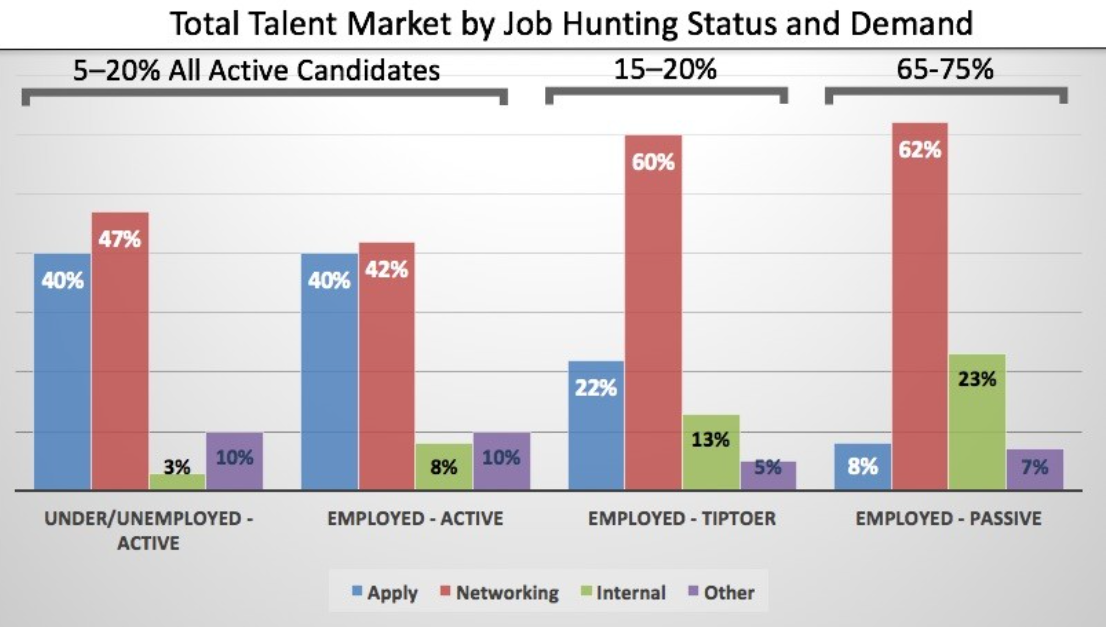
\includegraphics{figures/hiringpeople.bmp}
https://www.linkedin.com/pulse/new-survey-reveals-85-all-jobs-filled-via-networking-lou-adler/

Here we can see, that active candidates only represent 15-20 percent of the
entire jobmarket. Around 15-20 percent are only tiptoeing around the idea
of getting a new job, while the rest are passive candidates (meaning people who are
satisfied in their current position.).

Based on these graphs, we can see that at the very minimum, 42 percent of people are
hired based on networking, and that is only if you already have a job.
Whilst this percentage only goes up, the oppertunity for a job seeking person
to get hired based on an application only goes down. This reflects the
most effective way to get hired is through internal applications or networking.
On the flip side, it also nicely illustrates just how stiff competition there actually is,
if your only way of getting hired is through sending applications.

When you send out an application, there is an 8.3 percent probability, that
they will actually invite you to a job interview. Furthermore it takes around
10-15 interviews, before one gets a job offer. Obviously it varies depending
on educational background, job type and many other factors, but this is the average.
Some quick math ( (((100/8,3)*10)+((100/8,3)*15))/2 = 150..) tells us, that it will
take an average of 150 ish applications before one gets a job offer.
https://talent.works/2017/09/22/how-long-does-it-take-to-get-a-job-60-days-if-youre-in-hr-or-sales/

All these applications add up, before one can reap the reward. According to a
study conducted surveying 2000 Americans, by recruitment agency Randstad US
discovering the “art of the job hunt”, it takes an average of five
months from when the job search begins, until one actually lands
the job.
https://www.swnsdigital.com/2018/10/it-takes-5-months-of-searching-to-land-a-job-study-finds/

To add insult to injurry, after all the hard work of creating an application, it can
take quite some time before the hiring managers actually respond, that is if they ever
bother answering your application to begin with.
It takes around 3 days between they receive the application, before they answer.
This is the case for the most in demand roles in society, for the less in demand roles
such as writers, nurses and unskilled labour, it can be from 10 to over 30 days.
https://talent.works/2017/09/22/how-long-does-it-take-to-get-a-job-60-days-if-youre-in-hr-or-sales/
On average one can expect to hear back from employers within a week 41 percent
of the time. Within a couple of weeks 85 percent of the time.
https://www.indeed.com/career-advice/finding-a-job/how-long-should-you-wait-to-hear-back-about-a-job

Below some of the more popular jobs are illustrated as a function of interview
rate on the left and response delay on the left:
%\includegraphics{figures/interviewratexresponse delay.bmp}
https://talent.works/2017/09/22/how-long-does-it-take-to-get-a-job-60-days-if-youre-in-hr-or-sales/
The interview rate is further supported from a danish online survey, that concluded
that 65 percent of people get an interview within the first 15 applications and
 82.5 percent of people get an interview within the first 30 applications.
 https://get2business.wordpress.com/2009/10/27/hvor-mange-ans%C3%B8gninger-skal-der-til-for-at-fa-et-job/

\subsubsection{Optimize ones interview rate}
There are many factors to consider, if one wishes to optimize ones
chances of getting an interview, one of the more empirical proven ones
is what time and day one sends their application.
To get the highest chances, you have to apply between early Tuesday morning
and Thursday before noon using the employers local time. Monday is even better,
increasing your chances by 46 percent in regard to the average.
If one should apply on another day, the most important factor is that
it's done before 10AM, since the interview chances drops below 5 percent for
the majority of late evening pplications.
https://insights.dice.com/2019/10/30/best-times-days-submit-resume/

Perhaps one of the most influential condition of weither you get an interview,
is how fast you are at applying:
Based on 30000 datapoints from the company Speedrecruiters, you need
to apply within the first 14 days to have a practical chance of getting an
interview. it is such that 50 percent of the people who got an interview
for the job applied within the first week, and 75 percent of those who
got an interview applied within the first 14 days, whilst the chancess of
getting an interview thereafter dwindles exponentially.
https://www.jobfinder.dk/artikel/her-bedste-tidspunkt-at-sende-din-ansoegning/220987

Other factors that influenze the interview rate are as following:
1. Being a woman increases the chances by 48 percent.
2. Being older, but no older than 35, increases the interview rate by 25 percent.
3. Having more than one degree, increases ones chances by 22 percent.
4. Adding industry buzzwords increases your chances by 29 percent.
5. Demonstrate earlier job results using numbers increases chances by 40 percent.
6. Listing achievements, where you weren't in charge, but only a helping hand
 decreases your chances by 50 percent
7. Using leadership affiliated buzzwords increases your chances by 51 percent
8. Not using personal pronouns in the employment section increases your
chances by 55 percent.
9. Including a key skills section and buzzwords of the key skills increases your
 chances by 59 percent
10. Start ones sentences with distinct action verbs, increases ones chances by 140 percent.
Ptalent.works/2018/01/08/the-science-of-the-job-search-part-i-13-data-backed-ways-to-win/


%how long does it take to actually get a job

%how do these people then end up getting the job

%for the people sending applications, how many did they sen? ++ details

%best time to send applications, and why it can benefit people who
%dont have time there ++ howl ong should you wait with a followup

\subsection{Different expectations in a company}
Often in the different company's they have a different structure and information of what a CV could have in their application.
Most of the time the companies expectations can be related to work experience and education,
and a CV could either be long or short depends on which company the person is writing to. Some people can write a long CV,
but it isn't necessarily a good CV, and people can write a short one but it isn't good enough. 
Both of these statements could have some information that are not relevant to the company's requirement. Still there are some other
factors that can be included, and some companies´would love to know what the person did in that particular year. 
In that particular situation would be different from company to company, since those people who are working with humanities 
can have human related criteria for getting a job in this area. The same goes for IT where they have more work with a computer
than any other people, because these jobs immerse themselves everyday with it. According to Computerworld it-jobbank, 
they have actually analyzed a total 6700 job-advertisements in the year of 2015 and 2019 where the company was sorting all categories
that are related to IT, and they have published the top 10. It is shown between those years that the job-advertisements
have more of a technical and a more professional knowledgeable than before, since more
https://www.it-jobbank.dk/om-jobsoegning/karrierecenter/viden-om/it-karriere/disse-10-personlige-kompetencer-efterspoerger-virksomhederne?audiencetagid=140

Technical
Structured
Professional knowledge
Strong
Dynamic
Analytical
Responsible
Outgoing
Curious
Professional \\

Structured
Technical
Dynamic
Strong
Informal
Responsible
Professional
Outgoing
Analytical
Committed

Header: Include the Principal Investigator’s (PI’s) full name in the top left corner of the page header on every page. \\
Margins: Use at least half-inch margins. The header may fall within the top margin, but the body text should not begin closer than one half-inch from the edge of the page.
Font: Use size 11 Calibri for the main body of the text. Figures, tables and captions may be size 8 font.
Page Numbering: Each page must be numbered consecutively for each PDF upload. Each section of an uploaded document must begin with page 1.
Spacing: Use single spacing.
Document Format: Upload all attachments in PDF format.